\documentclass{standalone}
  \usepackage{tikz}
  \usetikzlibrary{arrows, automata, positioning}
  \tikzstyle{automaton}=[shorten >=1pt, pos=.4,
                         >=stealth', initial text=]
  \tikzstyle{accepting}=[accepting by arrow]

\begin{document}
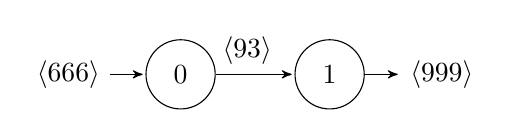
\begin{tikzpicture}[automaton]
  \node[state,initial,initial text=$\langle 666\rangle$] (0) {$0$};
  \node[state,accepting,accepting text=$\langle 999\rangle$] (1) [right=of 0] {$1$};
  \path[->] (0) edge node[above] {$\langle 93\rangle $} (1);
\end{tikzpicture}
\end{document}
